% Преамбула

\documentclass{article}

% Далее подключаем необходимые пакеты
\usepackage[utf8]{inputenc}
% Следующая группа пакетов делает возможным набор на русском языке.
\usepackage[T2A]{fontenc}
\usepackage[russian]{babel}
% Пакет для формирования автоматических отступов
\usepackage{indentfirst}
% Пакет для возможности работы с рисунками
\usepackage{graphicx}
% Сообщаем, в каком каталоге находятся изображения
\graphicspath{ {images/} }
% Пакет отвечает за изменение размеров полей и геометрии вывода на странице текста в целом
\usepackage[left=2cm, right=2cm, top=2cm, bottom=2cm, bindingoffset=0cm]{geometry}
% Пакет с цветами
\usepackage{xcolor}
% Это пакеты для печати кода в документе
\usepackage{listings}
% Настройки отображения листинга на Python
\definecolor{@clr-python-background}{RGB}{250,250,250}
\definecolor{@clr-python-text}{RGB}{0,0,0}
\definecolor{@clr-python-type}{RGB}{78,201,176}
\definecolor{@clr-python-func}{RGB}{255,127,0}
\definecolor{@clr-python-keyword}{RGB}{144,0,144}
\definecolor{@clr-python-comment}{RGB}{0,255,0}
% \definecolor{@clr-python-string}{RGB}{0,170,0}
% %\definecolor{@clr-python-preprocessor}{RGB}{0,0,153}
% \definecolor{@clr-python-definitions}{RGB}{0,0,255}

% \definecolor{@clr-python-variable}{RGB}{0,0,0}



\lstset{
    language=Python,
    tabsize=4,
    extendedchars=\true,
    keepspaces=true,
    breaklines,
    showstringspaces=\false,
    numbers=left,
    backgroundcolor=\color{@clr-python-background}
    basicstyle=\color{@clr-python-text},
    emph={int, float, complex, list, tuple, range, str, bytes, bytearray, memoryview, set, frozenset, dict, anext, ascii, bool, breakpoint, callable, chr, classmethod, compile, complex, divmod, enumerate, exec, filter, format, getattr, globals, hasattr, hash, help, hex, locals, map, object, oct, property, super, type, vars, zip},
    emphstyle={\color{@clr-python-type}},
    emph=[2]{abs, aiter, all, any, bin, delattr, dir, eval, exec, id, input, isinstance, issubclass, iter, len, max, min, next, open, ord, pow, print, repr, reversed, round, setattr, slice, sorted, staticmethod, sum, @classmethod, @staticmethod},
    emphstyle=[2]{\color{@clr-python-func}},
    keywordstyle=\color{@clr-python-keyword},
    morekeywords={as, False, None, True, assert, async, await, nonlocal, with, yield},
    commentstyle=\color{@clr-python-comment}
    }
% stringstyle=\color{@clr-python-string},
% commentstyle=\color{@clr-python-comment}\@twpythonfont,
    % identifierstyle=\color{@clr-python-variable}, 
    % emph=[2]{_, _PyBytes_, _PyInterpreterState_, _PyObject_, _PyTuple_, _Py_, _Py_c_, __, __PYVENV_LAUNCHER__, __abs__, __add__, __aenter__, __aexit__, __aiter__, __all__, __and__, __anext__, __annotations__, __args__, __await__, __bases__, __bool__, __breakpointhook__, __bytes__, __cached__, __call__, __callback__, __cause__, __ceil__, __class__, __class_getitem__, __classcell__, __closure__, __code__, __complex__, __concat__, __contains__, __context__, __copy__, __debug__, __deepcopy__, __defaults__, __del__, __delattr__, __delete__, __delitem__, __dict__, __dir__, __displayhook__, __divmod__, __doc__, __enter__, __eq__, __excepthook__, __exit__, __file__, __float__, __floor__, __floordiv__, __format__, __fspath__, __func__, __future__, __ge__, __get__, __getattr__, __getattribute__, __getitem__, __getnewargs__, __getnewargs_ex__, __getstate__, __globals__, __gt__, __hash__, __iadd__, __iand__, __iconcat__, __ifloordiv__, __ilshift__, __imatmul__, __imod__, __import__, __imul__, __index__, __init__, __init_subclass__, __instancecheck__, __int__, __interactivehook__, __inv__, __invert__, __ior__, __ipow__, __irshift__, __isub__, __iter__, __itruediv__, __ixor__, __kwdefaults__, __le__, __len__, __length_hint__, __loader__, __lshift__, __lt__, __main__, __matmul__, __missing__, __mod__, __module__, __mro__, __mul__, __name__, __ne__, __neg__, __new__, __next__, __not__, __notes__, __optional_keys__, __or__, __origin__, __package__, __parameters__, __path__, __pos__, __pow__, __prepare__, __qualname__, __radd__, __rand__, __rdivmod__, __reduce__, __reduce_ex__, __repr__, __required_keys__, __reversed__, __rfloordiv__, __rlshift__, __rmatmul__, __rmod__, __rmul__, __ror__, __round__, __rpow__, __rrshift__, __rshift__, __rsub__, __rtruediv__, __rxor__, __self__, __set__, __set_name__, __setattr__, __setitem__, __setstate__, __slots__, __spec__, __stderr__, __stdin__, __stdout__, __str__, __sub__, __subclasscheck__, __subclasses__, __subclasshook__, __suppress_context__, __total__, __traceback__, __truediv__, __trunc__, __unpacked__, __unraisablehook__, __xor__, _anonymous_, _b_base_, _b_needsfree_, _clear_type_, _current_, _emscripten_, _enter_, _field_, _fields_, _generate_next_value_, _get_child_, _get_preferred_, _ignore_, _leave_, _length_, _missing_, _numeric_repr_, _objects, _pack_, _register_, _type_, _unregister_},
    % emphstyle=[2]{\color{@clr-python-definitions}}


% Титульная часть добавляется в место документа, где находится команду \maketitle
\title{Конспект лекций по курсу:\\ "Алгоритмы и структуры данных"}
\author{Титов Василий Андреевич\thanks{Конспект составлен по материалам канала Серегея Балакириева (https://rutube.ru/channel/43304831/), конспекта лекций по АиСД 1-го курса ПМИ ФКН ВШЭ Михаила Густокашина (mgustokashin@hse.ru)}}
% Чтобы дата обновлялась автоматически надо заменить на \date\today
\date{Январь, 2026 г.}


% Начало нашшего документа, конец преамбулы
\begin{document}

% Эта команда создает титульную страницу
\maketitle

% Здесь будет автоматически генерироваться содержание документа
\tableofcontents

% Аннотация
\begin{abstract}
    Собственный конспект лекций по курсу алгоритмы и структуры данных применительно к языку программирования Python.
\end{abstract}

\section{Сложность алгоритмов}
\subsection{Проблемы при определении сложности}
    Алгоритм - набор инструкций для решения задачи.
    При написании программ возникает необходимость оценки качества алгоритма с точки зрения скорости вычислений и объёма потребляемой памяти.
Но для одного и того-же кода результат будет зависеть главным образом от следующих параметров:
\begin{itemize}
    \item "железа", на котором запускается программа
    \item объёма входных данных
\end{itemize}
Для исключения влияния первого пункта можно считать количество элементарных операций.
При этом вводятся некоторые упрощения.
Количество элементарных операций (скорость выполнения программ) или объём потребляемой памяти для $n$ 
входных данных равно значению функции $T(n)$ (для скорости и памяти могут быть разные функции и значения).

\subsection{Упрощения при определении сложности}

\subsection{Оценка сложности с позиции Big O (О-большое)}
$T(n)=O(g(n))$, если, начиная с некоторого $N_0$, $\forall$ $n$ $\exists$ некоторая константа $c$ такая, что 
выполняется равенство $T(n) \leq c * g(n)$.
Функция внутри $O(...)$ качественно показывает нам, как растёт сложность алгоритма по скорости или памяти при увеличении объёма входных данных.

\section{Основные структуры данных}
Структура данных - это способ организации хранения и доступа к данным.
\subsection{Статический массив}

\begin{figure}[h]
    \centering
    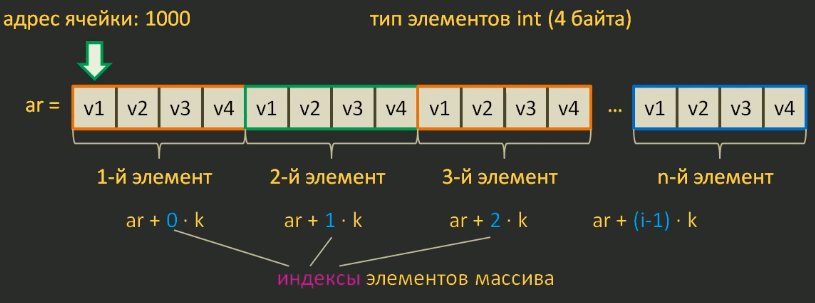
\includegraphics[width = 1\textwidth]{static_array.PNG}
    \caption{Структура статического массива}
    \label{fig:static_array_structure}
\end{figure}

Свойства:
\begin{enumerate}
    \item Фиксированный размер --> надо заранее знать $n$, иначе можем потерять данные.
    \item Значения элементов массива можно изменять.
    \item Все элементы массива одного типа данных --> размеры каждого элемента одинаковые.\label{prop:stat_arr_sametype}
    \item В памяти компьютера каждый элемент находится последовательно друг за другом, начиная с начала массива --> не всегда эффективно для больших $n$ и при вставке / удалении приходится сдвигать элементы\label{prop:stat_arr_seq}
    \item Благодаря свойствам \ref{prop:stat_arr_sametype} и \ref{prop:stat_arr_seq} доступ к $i$-му элементу статического массива $a$ осуществляется по формуле:
    \begin{equation}\label{eq:stat_arr_read}
        a[j] = a + j \cdot k = a[i - 1] = a + (i - 1) \cdot k,
    \end{equation}где $j$ -- индекс $i$-го элемента; $a$ -- адрес 1-го элемента c индексом 0; $k$ -- размер одного элемента.
\end{enumerate}

Незаполненные ячейки заполняются "мусором". Счётчик количества ячеек, в которых находится полезная информация, при добавлении или удалении 
элемента изменяется на +1 или -1 соответственно.

Сложность опреаций:
\begin{enumerate}
    \item Чтение и запись: $\Theta(1)$, следует из (\ref{eq:stat_arr_read})
    \item Вставка и удаление:
    \begin{enumerate}
        \item последнего элемента -- $O(1)$
        \item $i$-го элемента -- $O(n)$ из-за сдвига промежуточных элементов.
    \end{enumerate}
\end{enumerate}
В Python по умолчанию нет такой структуры.

\subsection{Динамический массив}

\begin{figure}[h]
    \centering
    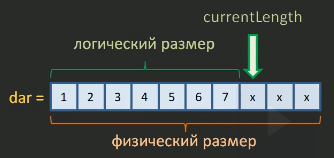
\includegraphics[width = 0.5\textwidth]{dinamic_array.PNG}
    \caption{Структура динамического массива}
    \label{fig:dinamic_array_structure}
\end{figure}

Свойства:
\begin{enumerate}
    \item Изменяемый размер --> если нужен $n$ (логический размер) > capacity (физический размер), то нужно расширить capacity --> следующая ячейка памяти может быть занята,
    поэтому перезаписываем данные в другую область памяти. Чтобы уменьшить вероятность повторного преезаписывания обычно в новой области capacity = $2 \cdot n$
    \item Значения элементов массива можно изменять.
    \item Все элементы массива одного типа данных --> размеры каждого элемента одинаковые. В списках Python для этого все элементы - это ссылки на объекты.\label{prop:din_arr_sametype}
    \item В памяти компьютера каждый элемент находится последовательно друг за другом, начиная с начала массива --> не всегда эффективно для больших $n$ и при вставке / удалении приходится сдвигать элементы. \label{prop:din_arr_seq}
    \item Благодаря свойствам \ref{prop:din_arr_sametype} и \ref{prop:din_arr_seq} доступ к $i$-му элементу динамического массива $a$ осуществляется по формуле:
    \begin{equation}\label{eq:din_arr_read}
        a[j] = a + j \cdot k = a[i - 1] = a + (i - 1) \cdot k,
    \end{equation}где $j$ -- индекс $i$-го элемента; $a$ -- адрес 1-го элемента c индексом 0; $k$ -- размер одного элемента.
\end{enumerate}

Незаполненные ячейки заполняются "мусором". Счётчик количества ячеек, в которых находится полезная информация, при добавлении или удалении 
элемента изменяется на +1 или -1 соответственно.

Сложность опреаций:
\begin{enumerate}
    \item Чтение и запись: $\Theta(1)$, следует из (\ref{eq:din_arr_read})
    \item Вставка:
    \begin{enumerate}
        \item последнего элемента, если нет переполнения -- $O(1)$
        \item последнего элемента, если есть переполнение -- $O(n)$ из-за перезаписи в другую облать памяти.
        \item $i$-го элемента -- $O(n)$ из-за сдвига промежуточных элементов.
    \end{enumerate}
    \item Удаление:
    \begin{enumerate}
        \item последнего элемента -- $O(1)$
        \item $i$-го элемента -- $O(n)$ из-за сдвига промежуточных элементов.
    \end{enumerate}
\end{enumerate}

\subsection{Односвязный список}

\begin{figure}[h]
    \centering
    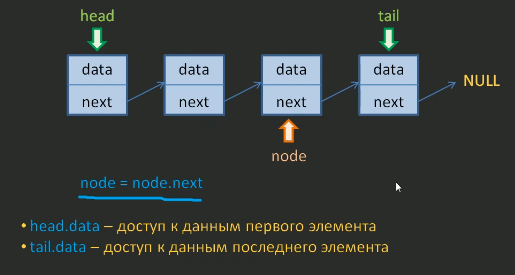
\includegraphics[width = 0.8\textwidth]{linked_list.PNG}
    \caption{Структура односвязного списка}
    \label{fig:linked_list_structure}
\end{figure}

Свойства:
\begin{enumerate}
    \item Изменяемый размер.
    \item Значения элементов массива можно изменять.
    \item Элементы могут находиться в памяти компьютера в неупорядоченном виде.\label{prop:link_list_separate} 
    \item Каждый элемент содержит ссылку на следующий элемент, а последний на None.\label{prop:link_list_refs} 
    \item Благодаря \ref{prop:link_list_separate} и \ref{prop:link_list_refs} можем расширять массив без перезаписи всех элементов при его заполнении.
\end{enumerate}

Храним в памяти адреса начала списка и конца. Если надо проитерироваться, то делаем это от начала.

Сложность опреаций:
\begin{enumerate}
    \item Чтение и запись:
    \begin{enumerate}
        \item последнего и первого элементов -- $O(1)$, т.к. храним указатели.
        \item $i$-го элемента -- $O(n)$, т.к. надо последовательно от начала по ссылкам добраться до $i$-го элемента.
    \end{enumerate} 
    \item Вставка:
    \begin{enumerate}
        \item последнего и первого элементов -- $O(1)$, т.к. храним указатели.
        \item $i$-го элемента -- $O(n)$, т.к. надо последовательно от начала по ссылкам добраться до $i$-го элемента.
    \end{enumerate}
    \item Удаление:
    \begin{enumerate}
        \item первого элемента -- $O(1)$
        \item последнего элемента -- $O(n)$, т.к. у указателя в конце нет ссылки на предыдущий элемент и надо итерироваться с самого начала.
        \item $i$-го элемента -- $O(n)$ т.к. надо последовательно от начала по ссылкам добраться до $i$-го элемента.
    \end{enumerate}
\end{enumerate}


\subsection{Двусвязный список}

\begin{figure}[h]
    \centering
    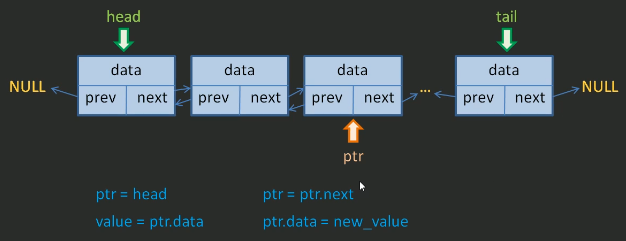
\includegraphics[width = 0.8\textwidth]{2linked_list.PNG}
    \caption{Структура двусвязного списка}
    \label{fig:2linked_list_structure}
\end{figure}

Свойства:
\begin{enumerate}
    \item Изменяемый размер.
    \item Значения элементов массива можно изменять.
    \item Элементы могут находиться в памяти компьютера в неупорядоченном виде.\label{prop:2link_list_separate} 
    \item Каждый элемент содержит ссылку на следующий и предыдущий элемент, а крайние на None.\label{prop:2link_list_refs} 
    \item Благодаря \ref{prop:2link_list_separate} и \ref{prop:2link_list_refs} можем расширять массив без перезаписи всех элементов при его заполнении.
    \item Благодаря \ref{prop:2link_list_refs} можем перемещать дополнительный указатель ptr в обе стороны --> быстро удалять элементы в конце списка.
\end{enumerate}

Храним в памяти адреса начала списка и конца.

Сложность опреаций:
\begin{enumerate}
    \item Чтение и запись:
    \begin{enumerate}
        \item последнего и первого элементов -- $O(1)$, т.к. храним указатели.
        \item $i$-го элемента -- $O(n)$, т.к. надо по ссылкам добраться до $i$-го элемента.
    \end{enumerate} 
    \item Вставка и удаление:
    \begin{enumerate}
        \item последнего и первого элементов -- $O(1)$, т.к. храним указатели и есть ссылки в обе стороны.
        \item $i$-го элемента -- $O(n)$, т.к. надо по ссылкам добраться до $i$-го элемента.
    \end{enumerate}
\end{enumerate}

В Python данная структура данных реализуется при помощи библиотеки collections и класса deque.


\subsection{Очередь (queue)}

Очередь - это не конкретная структура, как массивы или списки, а абстрактная структура. Суть её заключается в том, что мы работаем в основном с краевыми элементами, добавляем или удаляем их.
Соответственно, важными оказываются скорость доступа, вставки, удаления именно граничных элементов.
Работа с краевыми элементами может осуществляться по следующим правилам: 
\begin{itemize}
    \item FIFO (First-In-First-Out) -- классическая очередь. Новый элемент добавлется в конец, а извлекается элемент в из начала. 
Используется, например, при хранении заказов от клиентов интернет магазина или буфера данных. Такую очередь можно реализовать на базе двусвязного списка, т.к. мы работаем с обоими концами.
Очередь на базе двусвязного списка называют дэк (deque, double ended queue).
    \item LIFO (Last-In-First-Out) -- данный тип очереди ещё часто называют стеком. Хотя понятия стэка и очереди LIFO разные, в стэке мы работаем строго с элементами одного конца без доступа к $i$-му элементу,
    а в очереди нет (в основном с двух концов, но можем и обратиться к $i$-му). Новый элемент добавлется в конец, а извлекается элемент тоже с конца, т.е. работаем с одной стороны.
Используется, например, при хранении порядка вызова функций или сохранения предыдущих страничек в браузере, или анализе скобок в выражении. Такую очередь можно реализовать на базе статического/динамического массива (если работаем
только с последним элементом), на базе односвязного списка (работаем с первым элементом) или на базе двусвязного списка.
\end{itemize}

Свойства и сложность операций зависит от того, на базе какой структуры реализована очередь. При этом может использоваться гибридная структура из двусвязного списка и динамического массива.
Наличие динамического массива обеспечивает доступ к промежуточному элементу за О(1) внутри элемента двусвязного списка. Но есть и минус: более медленная вставка промежуточных элементов в начало элемента двусвязного списка (т.к. другие 
промежуточные элементы массива в списке приходится сдвигать) и в конец (т.к. можем уйти в перезапись).

\begin{figure}[h]
    \centering
    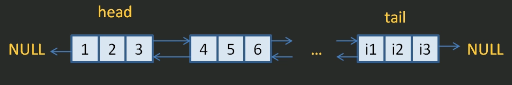
\includegraphics[width = 0.8\textwidth]{hybrid_queue.PNG}
    \caption{Структура гибридной очереди}
    \label{fig:hybrid_queue}
\end{figure}

В Python данная структура данных реализуется при помощи библиотеки collections и класса deque.

\paragraph{Примеры задач}
Рассмотрим решение нескольких типовых задач на Python.
\lstinputlisting{structure_tasks/stack_psp.py}
\lstinputlisting{structure_tasks/stack_shunting_yard.py}
\lstinputlisting{structure_tasks/stack_calculate_expression.py}
\lstinputlisting{structure_tasks/deque_min_in_window.py}




\subsection{Бинарные деревья (binary tree)}

\begin{figure}[h]
    \centering
    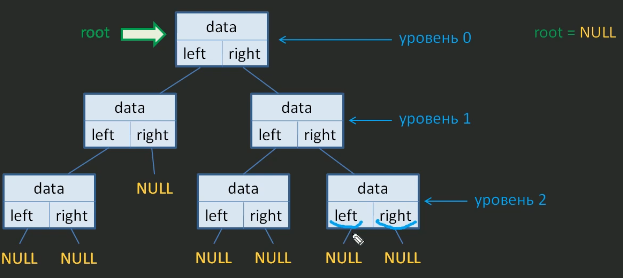
\includegraphics[width = 0.8\textwidth]{bin_tree_struct.PNG}
    \caption{Структура бинарного дерева}
    \label{fig:bin_tree_struct}
\end{figure}

Дерево применяется, когда надо обрабатывать иерархические структуры данных: каталоги или генеологическое дерево.

Бинарное дерево -- дерево, у вершин которого не более 2-х потомков

Вершина (node) -- узел, у которого есть родитель и потомок.

Корень (root) -- узел, у которого отсутствует родитель.

Лист -- узел, у которого нет ни одного потомка.

Сбалансированное дерево -- дерево, у которого поддеревья от одной вершины отличаются не больше, чем на один уровень.

На вершину дерева ведёт указатель. В каждом узле имеется 3 поля: значение узла (data), ссылки на левого и правого потомков. Иногда хранится ссылка на родителя.
На практике стараются свести дерево к бинарному дереву и сбалансировать его.

Для решения определённого класса задач формируют бинарное дерево по следующим правилам:
\begin{enumerate}
    \item Если добавляемый элемент меньше data в родительском узле, то он уходит в левую ветвь.
Если добавляемый элемент больше data в родительском узле, то он уходит в правую ветвь.
    \item Если добавляемый элемент равен data в родительском узле, то он не добавляется в дерево.
\end{enumerate}

Способы обхода:
\begin{itemize}
    \item Обход в ширину (breadth-first). Пробегаемся по каждому узлу на уровне слева направо.
    \item Обход в глубину. Пробегаемся по каждому узлу сверху вниз. Если сформировали дерево по правилам выше, то
при обходе в глубину в порядке LNR всегда будем получать возрастающую последовательность. При проходе в порядке RNL
последователльность будет убвающей.
\end{itemize}

Сложность опреаций:
\begin{enumerate}
    \item Поиск:
    \begin{enumerate}
        \item В худшем случае, когда $n$ упорядочены: $O(n)$
        \item На сбалансированном дереве: $O(log_2 n)$
    \end{enumerate}
\end{enumerate}

Методы балансировки двоичных деревьев:
\begin{itemize}
    \item АВЛ-дерево;
    \item красно-чёрное дерево;
    \item расширяющееся или косое дерево (splay tree)
\end{itemize}

Удаление вершин:
\begin{itemize}
    \item Удаляем лист. Просто у родителя убираем ссылку на потомка.
    \item Удаляем узел $a$ с одним потомком $b$. Просто у родителя вместо ссылки на удаляемого потомка $a$ вставляем ссылку на $b$.
    \item Удаляем узел с двумя потомками. Сам узел не удаляется, а меняется значение. Новое значение -- наименьшее значение из правой ветви.
В общем случае нужно 3 указателя: на удаляемый узел, на узел с наименьшим значением и на узел-родителя узла с наименьшим значением.
\end{itemize}

Пример реализации бинарного дерева на Python.
\lstinputlisting{structure_tasks/binary_tree.py}

\subsection{Куча (heap)}

Куча представляет собой бинарное дерево. Значение в каждом узле кучи минимумов меньше (для кучи максимумов больше), чем значения каждого потомка.
Кучу стараются заполнить плотно.




\subsection{Хэш-таблицы}
Хэш таблица представляет собой комбинацию динамического массива и специальной хэш-функции $h(k)$. Каждому индексу $i$ массива соответствует пара ключ-значение.
Хэш-функция - алгоритм преобразования ключа $k$ в индекс массива $i$.
Порядок заполнения хэш таблицы: ключ --> некая специальная функция --> число $k$ --> хэш-функция --> индекс массива --> (ключ-значение).
Требования к "хорошей" хэш-функции:
\begin{itemize}
    \item Детерминированность -- одному и тому же ключу $k$ соответствует один и тот же индекс $i$ хэш-таблицы. Разным ключам $k$ соответствуют разные индексы $i$.
Т.к. ключей намного больше, чем $m$, то для одного и того же ключа могут получаться одинаковые индексы $i$ -- коллизия.
    \item Высокая скорость вчисления $i$.
    \item Полученный индекс $i$ должен быть в пределах от 0 до $m - 1$.
    \item Хэш таблица должна заполняться равномерно, чтобы уменьшить вероятность появления коллизий. В этом случае средняя длина
    цепочек при коллизии будет равна $\alpha$.
\end{itemize}
Есть понятие $\alpha = n / m$ -- степень заполненности. $n$ -- количество ключей в таблице, $m$ -- количество ячеек. $\alpha < 1$ -- есть свободные ячейки. $\alpha = 1$ -- нет свободных ячеек.
$\alpha > 1$ -- все ячейки заполнены и есть коллизии.

Методы построения хэш-функции:
\begin{itemize}
    \item Метод деления: $h(k) = k \% m$. Если $m$ -- степень 2, то возникает проблема как на рисунке \ref{fig:hash_func_mod}. Чтобы избежать этого эффекта число $m$ нужно выбирать простым и далёким от степени 2 --> неудобно.
    \begin{figure}[h]
        \centering
        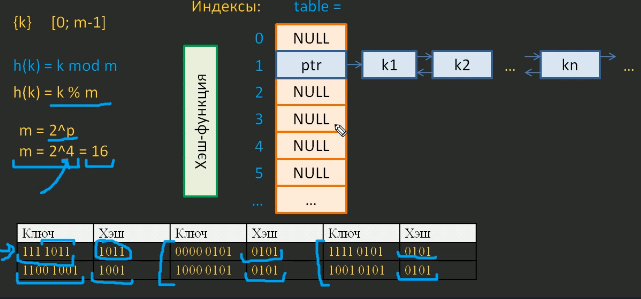
\includegraphics[width = 0.8\textwidth]{hash_func_mod.PNG}
        \caption{Иллюстрация недостатка хэш-функции $h(k) = k \% m$}
        \label{fig:hash_func_mod}
    \end{figure}
    \item Метод умножения: $h(k) = floor(m \cdot [(k \cdot A) \% 1])$, где $A$ -- константа от 0 до 1; floor - округление до наименьшего целого.
    Теперь нет ограничений на m. Но как выбрать $A$? Дональд Кнут предложил принять $A = (\sqrt{5} - 1) / 2 = 0,61803...$
    \item SHA -- семейство алгоритмов хэширования;
    \item CRC -- циклический избыточный код;
    \item MD5 -- 128-битный алгоритм хэширования.
    \item Универсальное хэширование
\end{itemize}

Как бы хорошо не работал алгоритм хэширования для конкретной $h(k)$ можно подобрать такой набор $k$, что алгоритм хэширования будет давать один и тот же $i$.
Этим могу воспользоваться злоумышленники. Чтобы исключить предсказуемость распределения ключей по индексам таблицы для вновь создаваемой хэш-таблицы используют одну случайную хэш-функцию из набора $\{h_1(k), h_2(k)..., h_H(k)\}$.
В этом наборе для каждой функции при подаче определённого набора $k$ должны формироваться разные наборы $i$.
Указанный набор $\{h_1(k), h_2(k)..., h_H(k)\}$ называется универсальным. Томас Кормен предложил следующий способ создания универсального набора. Правило, по которому составляется хэш-функция:
\begin{equation}\label{eq:univers_set_hash}
        h_{ab}(k)=([a \cdot k + b] \% p) \% m,
\end{equation}где $p > m$ -- простое число, $a, b$ -- константы, выбранные случайным образом из наборов $\{1, 2, 3 ... p - 1 \}$, $\{0, 1, 2 ... p - 1 \}$ соответственно.

Хэш функция, построенная по такому правилу, для разных ключей выдаст один и тот же индекс с вероятностью $1/m$. 
Количество хэш-функий в наборе равно $p(p-1)$. Значение $m$ выбирается произвольно. 


Методы хранения данных в хэштаблицах и способы разрешения коллизий:
\begin{itemize}
    \item Метод цепочек. Каждый элемент массива содержит ссылку на двусвязный список с парами ключ-значение. Если после работы хэш-функции получился уже занятый индекс, то
    проваливаемся в двусвязный список и добавляем новую пару ключ-значение. Может получаться длинная цепочка в ячейке.
    Сложность операций:
    \begin{enumerate}
        \item Доступ:
        \begin{enumerate}
            \item Если в ячейке нет коллизии: $O(1)$
            \item Если в ячейке есть коллизия: $O(1 + \alpha)$.
        \end{enumerate}
        \item Вставка:
        \begin{enumerate}
            \item Коэффициент $\alpha$ меньше порога перезаписи и нет колизии: $O(1)$;
            \item Коэффициент $\alpha$ меньше порога перезаписи и есть колизия: $O(1 + \alpha)$;
            \item Если уходим в перезапись: $O(n)$. Если при добавлении нового элемента коэффициент $\alpha$ больше порога перезаписи, то:
            \begin{enumerate}
                \item Выделяем в памяти в два раза больше ячеек.
                \item Перезаписываем уже записанные пары ключ-значение. Это нужно, т.к. размеры таблицы изменились и индексы у существующих данных могут измениться.
            \end{enumerate} 
        \end{enumerate}
        \item Удаление:
        \begin{enumerate}
            \item Если в ячейке нет коллизии: $O(1)$
            \item Если в ячейке есть коллизия: $O(1 + \alpha)$
        \end{enumerate}
    \end{enumerate}
    \item Метод открытой адресации. В ячейках массива хранятся ссылки на пары ключ-значение. В незаполненных ячейках None. Такой способ применяется в Python.
    \begin{itemize}
        \item Линейное исследование. Формирование хэш-функции:
        \begin{equation}\label{eq:hash_linear}
            h(k, j) = (h^{'}(k) + j) \% m,
        \end{equation}где $h^{'}(k)$ -- исходная хэш-функция; $h(k)$ -- результирующая хэш-функция; $j$ -- счётчик, изначально равен 0.

        При добавлении нового значения если ячейка занята, то переходим к следующей, увеличивая счётчик $j$ на 1. И так, пока не встретим None.
        При удалении в ячейки оставляем метку 'deleted'. Это надо, чтобы при поиске ключей за удалённым значением, мы не остановили поиск раньше времени.
        Могут образовываться длинные цепочки и неравномерность.
        \item Квадратичное исследование.
        \begin{equation}\label{eq:hash_squad}
            h(k, j) = (h^{'}(k) + a \cdot j + b \cdot j^2) \% m,
        \end{equation}где $h^{'}(k)$ -- исходная хэш-функция; $h(k, j)$ -- результирующая хэш-функция; $j$ -- счётчик, изначально равен 0; $a, b$ -- константы.
        Здесь плюс в том, что образуются более короткие последовательности ячеек. Константы $a, b, m$ должны быть подобраны так, чтобы $h(k, j)$ перебирала все ячейки ровно 1 раз.
        \item Двойное хэширование.
        \begin{equation}\label{eq:hash_double}
            h(k, j) = (h^{'}(k) + j \cdot g(k)) \% m,
        \end{equation}где $h^{'}(k)$ -- исходная хэш-функция; $h(k, j)$ -- результирующая хэш-функция; $j$ -- счётчик, изначально равен 0;
        $g(k)$ -- вспомогательная хэш-функция. Такой способ позволяет хорошо перемешивать ключи.
        Значения $g(k)$ и $m$ должны быть взаимно простыми, иначе при разрешении коллизии можем попадать на одни и те же индексы. Томасом Корманом
        предложена следующая вспомогательная хэш-функция:
        \begin{equation}\label{eq:hash_double_help}
            g(k) = 1 + k \% m',
        \end{equation}где $m' = m - 1$.
        Сложность операций при использовании двойного хэширования:
        \begin{enumerate}
            \item Доступ, вставка, удаление в среднем за $O(1)$
        \end{enumerate}
    \end{itemize}
\end{itemize}


В Python по принципу хэш-таблиц работает два типа данных: словарь (dict) и множество (set). Словарь -- классическая хэш-таблица.
Множество в Python -- это та же хэш-таблица, все значения которой равны None.
Ключи dict или элементы set должны быть хэшируемыми --> неизменяемыми типами данных.


\section{Алгоритмы сортировки}


\subsection{Медленные сортировки}

\subsubsection{Сортировка пузырьком (bubble sort)}
\lstinputlisting{sorts/sort_bubble.py}

\subsubsection{Сортировка вставками (insertion sort)}
\lstinputlisting{sorts/sort_insertion.py}

\subsubsection{Сортировка выбором (selection sort)}
\lstinputlisting{sorts/sort_selection.py}

\subsubsection{Сравнение медленных сортировок}
Сортировка называется устойчивой, если она сохраняет взаимный порядок одинаковых элементов.

\begin{figure}[h]
    \centering
    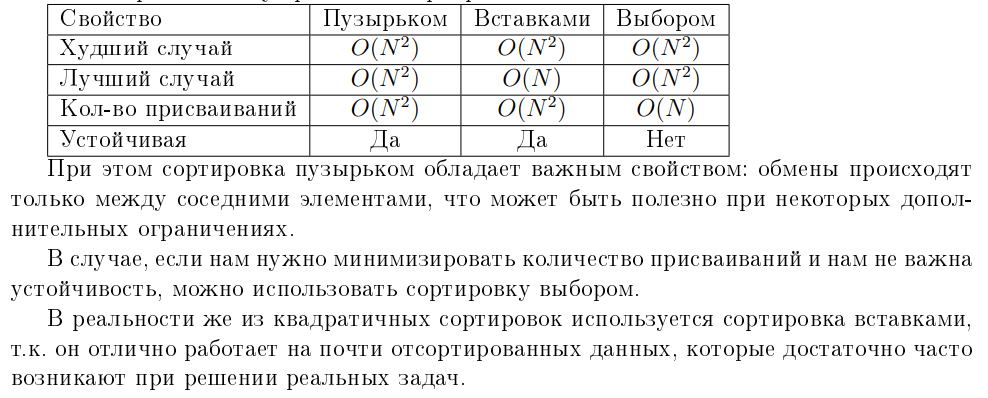
\includegraphics[width = 0.8\textwidth]{sorts_compare.PNG}
    \caption{Сравнение квадратичных сортировок}
    \label{fig:sorts_squad_compare}
\end{figure}




\subsection{Быстрые сортировки}

\subsubsection{Сортировка слиянием (merge sort)}
\lstinputlisting{sorts/sort_merge.py}


\subsubsection{Сортировка Хоара}



\section{Дополнительные материалы}
ВШЭ, лекции Густокашина
ФПМИ МФТИ
Яндекс хендбук,
Яндекс тренировки
Искусство программировать, Дональд Кнут
Алгоритмы: построение и анализ, Томас Кормен
\end{document}


